\subsection{Sensors}
    \subsubsection{GPS Receivers}
        % Properties:
        % \begin{itemize}
        %     \item update rate
        %     \item reference location
        %     \item horizontal position accuracy
        %     \item vertical position accuracy
        %     \item velocity accuracy
        %     \item decay factor ?
        %     \item failure rate?
        % \end{itemize}

        The \ac{gps} is a \ac{gnss} owned adn operated by United States government. It allows for determining position, velocity and time using data taken from at least four \ac{gps} satellites.

        Previously using \ac{gps} receivers in \ac{leo} was burdened with technical challenges, as off-the-shelf components were mostly designed for terrestial operations, not encompassing for example for large variations in the received signal Doppler frequencies. Recently smaller \ac{gps} receivers became available, even for CubeSat use, such as \textit{Venus838FLPx GPS Receiver}\cite{gpsdatasheet}, allowing for real time orbit determination using \ac{gps} navigation in smaller satellite projects.\cite{gomes2007real} When choosing a \ac{gps} receiver one must take several parameters into consideration:
        
        \begin{itemize}
            \item Update rate
            \item Horizontal position accuracy
            \item Vertical position accuracy
            \item Velocity accuracy
            \item Decay factor?
            \item Failure rate?
        \end{itemize}

        All listed parameters are set up in \ac{scars} \textit{GPS Receiver} part, but rather than designing a model from scratch a MATLAB's Navigation Toolbox function, \verb|gpsSensor| was nested inside a masked Simulink block.


    \subsubsection{Accelerometers}
        % accelerometer misalignment

    \subsubsection{Magnetometers}
        % accelerometer misalignment


    \subsubsection{Gyroscopes}
        % https://www.youtube.com/watch?v=anMzEbbbrp8
        % Parameters:
        % \begin{itemize}
        %     \item change over temperature
        %     \item zero rate level change over temperature [dps/*C] (but this can biased to get rid of the error, so is not necessary to model)
        %     \item senistivity
        %     \item Measurement range
        %     \item Angle Random Walk (same Parameter as FFT and Power Spectral Density)
        % \end{itemize}

        Gyroscopes, which fall under category of inertial sensors, measure angular rate around fixed axis. In smaller spacecraft, which is in great deal of \ac{scars} toolbox use-cases, the conventional spinning mass gyroscopes are rarely used, due to limitations in mass and size. Recent developments allow for use of much smaller and cheaper \ac{mems} gyroscopes, which are vibrating angular rate sensors. They were chosen to model for the toolbox, as of popularity in projects with highly restricted budget. \cite{armenise2010advances} Inside of vibrating gyroscope the Coriolis effect is a cause the vibrating core to produce a force acting on its support. The measurement of the force is used to determine the rate of rotation of the body around gyroscope axis. \ac{mems} gyros are similar to integrated circuits, which use the miniaturized version of mechanisms based on principles of operation of either vibrating wheels, tuning forks, resonant solids or similar common designs. \cite{bernstein2003overview} While, besides previously mentioned qualities, the upsides of \ac{mems} gyroscopes are availability of both analog and digital outputs, low power consumption and commercial availability. On the other hand, \ac{mems} gyros have shorter lifetime and lower performance when compare to pricier alternatives.

        \begin{figure}[H]
            \centering
            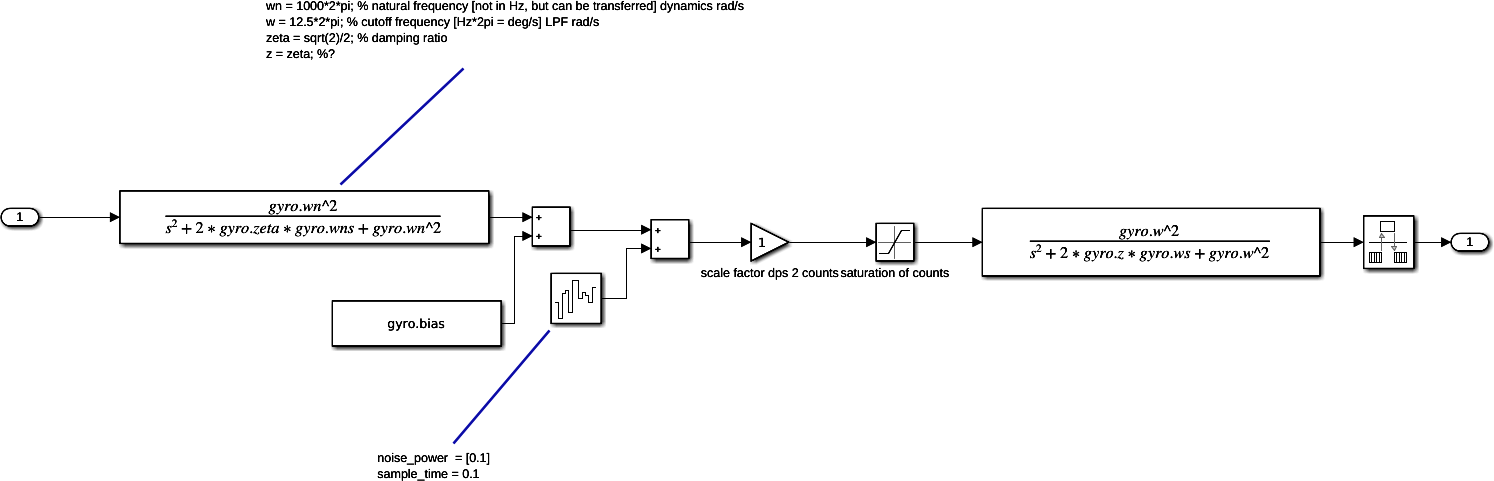
\includegraphics[width=1\textwidth]{2-toolbox/gyros.png}
            \caption{Gyroscope model}
            \label{fig:gryo_simulink}
        \end{figure}

        In the toolbox the following sources of gyroscope errors are modeled:
        \begin{itemize}
            \item Bias offset:
            \item Scale factor: 
            \item \ac{arw}: A high frequency noise term that has a correlation time much shorter than the sample time. Can be defined as white noise component on the sensor output. Specified either in $\frac{deg}{\sqrt{h}}$ or, as a power spectral density, in $\frac{(deg/h)^2}{Hz}$. % cite this here: http://citeseerx.ist.psu.edu/viewdoc/download?doi=10.1.1.210.1133&rep=rep1&type=pdf
            \item Quantization Error: An error which is caused by the digital quantization of output signal, obtained when sampling analog input.
            \item ...
        \end{itemize}

       - Cite this: \cite{kapeelmodeling} % for errors

    % \subsubsection{Inertial Measurement Units}

